\documentclass{article}
\usepackage[utf8]{inputenc}

\title{Computación Distribuida \\ Tarea 05}
\author{Olea Olvera Marco Iván \\ Arteaga Hernández Alejandro Iabin}
\date{}

\usepackage[top=1.5cm, bottom=1.5cm, left=2cm, right=2cm]{geometry}
\usepackage{tikz}
\usepackage{fouriernc}
\usepackage{amssymb}
\usepackage{listings}
\usepackage{amsmath}
\lstset{
  basicstyle=\ttfamily,
  mathescape
}

\usepackage{graphicx}
\graphicspath{{./}}

\begin{document}

\maketitle

\section{}
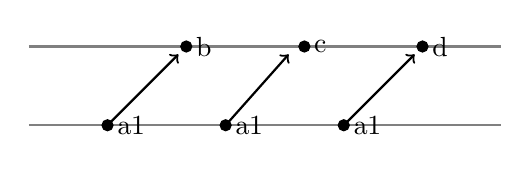
\begin{tikzpicture}

\draw[gray, thick] (-1,1) -- (5,1);
\draw[gray, thick] (-1,0) -- (5,0);

\filldraw[black] (0,0) circle (2pt) node[anchor=west] {a1};
\draw[thick,->] (0,0) -- (0.9,0.9);

\filldraw[black] (1,1) circle (2pt) node[anchor=west] {b};

\filldraw[black] (1.5,0) circle (2pt) node[anchor=west] {a1};
\draw[thick,->] (1.5,0) -- (2.3,0.9);
\filldraw[black] (2.5,1) circle (2pt) node[anchor=west] {c};

\filldraw[black] (3,0) circle (2pt) node[anchor=west] {a1};
\draw[thick,->] (3,0) -- (3.9,0.9);
\filldraw[black] (4,1) circle (2pt) node[anchor=west] {d};
\end{tikzpicture}
\\
$a_1 \underset{s}{=>} a_2$\\
$a_2 \underset{s}{=>} a_3$\\
$a_1 \underset{s}{=>} a_3$\\
$a_1 \underset{s}{=>} b$\\
$a_1 \underset{s}{=>} c$\\
$a_1 \underset{s}{=>} d$\\
$a_2 \underset{s}{=>} c$\\
$a_2 \underset{s}{=>} d$\\
$a_3 \underset{s}{=>} d$\\

Termina en a lo más $T+T+T+D$\\
son el tiempo que se tarda en ser mandado cada mensaje más el tiempo máximo que puede tardar el último mensaje en llegar, como todos se pueden tardar D tiempo máximo en llegar, entonces el D del último mensaje puede ser el último en llegar
\section{}
$Z(c) \leq  B_{ab}+B_{bc}$\\
$Z(e) \leq  B_{ab}+B_{bc}+ B_{cd}+B_{de}$\\
los sumamos de cada lado
$Z(e) - Z(c) \leq B_{ab}+B_{bc}+ B_{cd}+B_{de} - B_{ab}-B_{bc} $\\
$Z(e) - Z(c) \leq B_{cd}+B_{de} $

Es la suma de los retardos mínimos de cada mensaje\\
$B_{ba}+B_{cb}+B_{dc}+B_{ed}$.

Reloj lógico\\\\
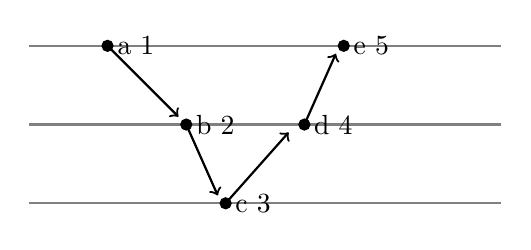
\begin{tikzpicture}
\draw[gray, thick] (-1,2) -- (5,2);
\draw[gray, thick] (-1,1) -- (5,1);
\draw[gray, thick] (-1,0) -- (5,0);

\filldraw[black] (0,2) circle (2pt) node[anchor=west] {a 1};
\draw[thick,->] (0,2) -- (0.9,1.1);

\filldraw[black] (1,1) circle (2pt) node[anchor=west] {b 2};
\draw[thick,->] (1,1) -- (1.4,0.1);
\filldraw[black] (1.5,0) circle (2pt) node[anchor=west] {c 3};
\draw[thick,->] (1.5,0) -- (2.3,0.9);
\filldraw[black] (2.5,1) circle (2pt) node[anchor=west] {d 4};
\draw[thick,->] (2.5,1) -- (2.9,1.9);
\filldraw[black] (3,2) circle (2pt) node[anchor=west] {e 5};
\end{tikzpicture}.


Reloj lógico\\\\
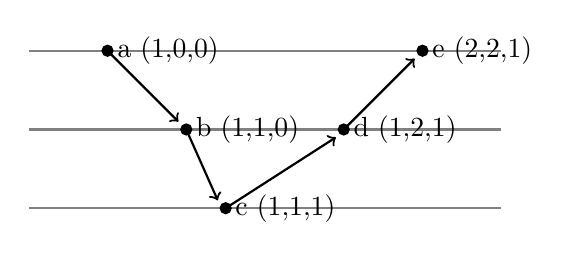
\begin{tikzpicture}
\draw[gray, thick] (-1,2) -- (5,2);
\draw[gray, thick] (-1,1) -- (5,1);
\draw[gray, thick] (-1,0) -- (5,0);

\filldraw[black] (0,2) circle (2pt) node[anchor=west] {a (1,0,0)};
\draw[thick,->] (0,2) -- (0.9,1.1);

\filldraw[black] (1,1) circle (2pt) node[anchor=west] {b (1,1,0)};
\draw[thick,->] (1,1) -- (1.4,0.1);
\filldraw[black] (1.5,0) circle (2pt) node[anchor=west] {c (1,1,1)};
\draw[thick,->] (1.5,0) -- (2.9,0.9);
\filldraw[black] (3,1) circle (2pt) node[anchor=west] {d (1,2,1)};
\draw[thick,->] (3,1) -- (3.9,1.9);
\filldraw[black] (4,2) circle (2pt) node[anchor=west] {e (2,2,1)};
\end{tikzpicture}
\section{}

suponemos que $\varphi_1$ no pasó antes que $\varphi_2$
\\
$\varphi_1$ y $\varphi_2$ son de procesos diferentes $p$ y $p'$\\
Para $LT(\varphi_1) < LT(\varphi_2)$ debemos de tener 
forzosamente  que 
\\$LT(\varphi_1)_p < LT(\varphi_2)_p$\\
Pero esto solo sucede si $LT(\varphi_1)$ está propagado a p', para alguna secuencia de mensajes, que inician en p y terminan en p' antes de que $\varphi_2$ ocurra, por lo tanto $\varphi_1$ y $\varphi_2$ son comparables, y en este caso $\varphi_1$  pasó antes que $\varphi_2$

\end{document}
